\section{The Well}
{{\footnotesize
\begin{description}[labelwidth=5em, labelsep=1em, leftmargin=*, align=left, itemsep=0.3em, parsep=0em]
  \item[date:] 2024-12-03
  \item[version:] TODO
  \item[last\_updated:] 2025-06
  \item[expired:] unknown
  \item[valid:] yes
  \item[valid\_date:] TODO
  \item[url:] \href{https://polymathic-ai.org/the\_well/}{https://polymathic-ai.org/the\_well/}
  \item[doi:] TODO
  \item[domain:] biological systems, fluid dynamics, acoustic scattering, astrophysical MHD
  \item[focus:] Foundation model + surrogate dataset spanning 16 physical simulation domains
  \item[keywords:]
    - surrogate modeling
    - foundation model
    - physics simulations
    - spatiotemporal dynamics
  \item[summary:] A 15 TB collection of ML-ready physics simulation datasets (HDF5), covering 16 domains-from biology to astrophysical magnetohydrodynamic simulations-with unified API and metadata. Ideal for training surrogate and foundation models on scientific data. :contentReference[oaicite:1]\{index=1\}

  \item[licensing:] TODO
  \item[task\_types:]
    - Supervised Learning
  \item[ai\_capability\_measured:]
    - Surrogate modeling
    - physics-based prediction
  \item[metrics:]
    - Dataset size
    - Domain breadth
  \item[models:]
    - FNO baselines
    - U-Net baselines
  \item[ml\_motif:]
    - Foundation model, Surrogate
  \item[type:] Dataset
  \item[ml\_task:]
    - Supervised Learning
  \item[solutions:] TODO
  \item[notes:] Includes unified API and dataset metadata; see 2025 NeurIPS paper for full benchmark details. Size: 15 TB. :contentReference[oaicite:2]\{index=2\}

  \item[contact.name:] Wes Brewer
  \item[contact.email:] unknown
  \item[datasets.links.name:] 16 simulation datasets
  \item[datasets.links.url:] \href{HDF5) via PyPI/GitHub}{HDF5) via PyPI/GitHub}
  \item[results.links.name:] ChatGPT LLM
  \item[fair.reproducible:] Yes
  \item[fair.benchmark\_ready:] Yes
  \item[ratings.software.rating:] 0
  \item[ratings.software.reason:] Not analyzed.

  \item[ratings.specification.rating:] 7.0
  \item[ratings.specification.reason:] Explores LLM understanding of mental health scenarios; framing is creative but loosely defined.

  \item[ratings.dataset.rating:] 6.0
  \item[ratings.dataset.reason:] Dataset is described in concept but not released; privacy limits public access though synthetic proxies are referenced.

  \item[ratings.metrics.rating:] 7.0
  \item[ratings.metrics.reason:] Uses manual annotation and quality scores, but lacks standardized automatic metrics.

  \item[ratings.reference\_solution.rating:] 6.0
  \item[ratings.reference\_solution.reason:] Provides few-shot prompt examples and human rating calibration details.

  \item[ratings.documentation.rating:] 5.0
  \item[ratings.documentation.reason:] Paper gives use cases, but code and data are not yet public.

  \item[id:] the\_well
  \item[Citations:] \cite{neurips2024_4f9a5acd}
  \item[Ratings:]
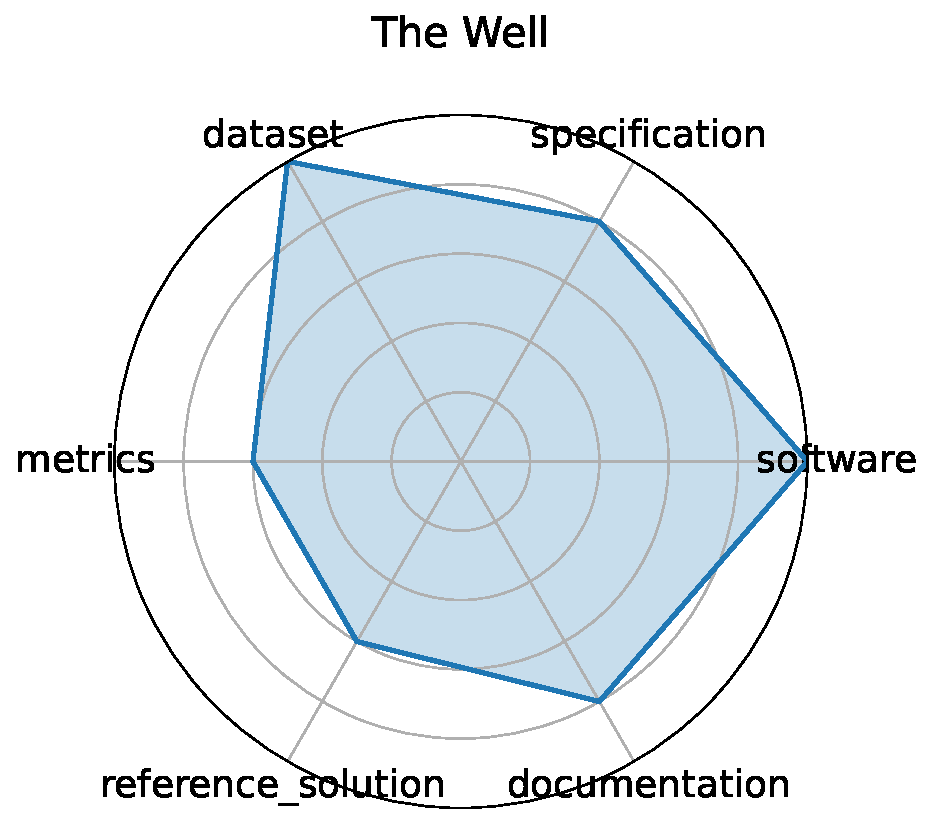
\includegraphics[width=0.2\textwidth]{the_well_radar.pdf}
\end{description}
}}
\clearpage